\documentclass[10pt,a4paper]{article}

\newcommand{\cvRolle}{Senior Cloud Infrastructure \& DevOps Engineer}
\newcommand{\cvSubheader}{CI/CD Automation $\cdot$ Release Optimization $\cdot$ Platform Engineering Specialist}

% ==========================================
% SETTINGS.TEX - ZENTRALE KONFIGURATION
% ==========================================
\usepackage[utf8]{inputenc}
\usepackage[T1]{fontenc}
\usepackage[american]{babel}
\usepackage[top=1.8cm, bottom=1.8cm, left=1.8cm, right=1.8cm]{geometry}
\usepackage{xcolor}
\usepackage{hyperref}
\usepackage{enumitem}
\usepackage{graphicx}
\usepackage{calc}
\usepackage{charter}
\usepackage{microtype}
\usepackage{etoolbox}

% --- DESIGN FARBEN ---
\definecolor{primary}{RGB}{15, 23, 42}      % Deep Slate / Tech Dark
\definecolor{accent}{RGB}{37, 99, 235}     % MP Blue Accent
\definecolor{textgray}{RGB}{51, 65, 85}    % Charcoal Body Text

% --- PERMANENTE ABSENDER-DATEN ---
\newcommand{\meinName}{Markus Gruber, M.Sc.}
\newcommand{\meineStrasse}{Maximilianstraße 55 Stg. B 20}
\newcommand{\meinOrt}{3100 St. Pölten}
\newcommand{\meineEmail}{Markus.Gruber4@gmx.net}
\newcommand{\meineTel}{+43 650 5871145}
\newcommand{\meinLinkedin}{https://www.linkedin.com/in/markus-gruber-70851428/}
\newcommand{\meinGithub}{https://github.com/CodeByMaxx}

% --- ROLLEN-DEFAULTS ---
\providecommand{\cvRolle}{}
\renewcommand{\cvRolle}{AI & Automation Engineer -- M&A Deal Automation}
\providecommand{\cvSubheader}{}
\renewcommand{\cvSubheader}{Python \cdot LLM APIs (OpenAI, Anthropic) \cdot Financial Data Pipelines \cdot Agent Workflows \cdot RAG}

% --- EMPFÄNGER-DATEN ---
\newcommand{\firmenName}{MP Corporate Finance}
\newcommand{\ansprechPartner}{Katharina Schwarzl-Moser (HR Manager)}
\newcommand{\firmenStrasse}{Wien, Österreich}
\newcommand{\firmenOrt}{Wien, Österreich}

% --- INTELLIGENTE ADRESS-AUSGABE (Verhindert doppelte Zeilen, wenn Straße == Ort) ---
\newcommand{\firmenAdresse}{%
    \def\tempStrasse{Wien, Österreich}%
    \def\tempOrt{Wien, Österreich}%
    \ifx\tempStrasse\tempOrt
        \tempOrt%
    \else
        Wien, Österreich \\[0.15em] Wien, Österreich%
    \fi
}

\newcommand{\stellenTitel}{AI & Automation Engineer (f/m/x)}
\newcommand{\referenzNummer}{}

\newcommand{\anrede}{Dear Ms. Schwarzl-Moser,}
\newcommand{\firmenHighlight}{MP Corporate Finance is one of Europe's leading mid-market M&A boutiques, where your AI tools will be deployed on live cross-border transactions from day one.}

% --- HEADER BEFEHL ---
\newcommand{\cvHeader}{%
\begin{center}
    {\Huge\bfseries\color{primary} \meinName}\\[0.1cm]
    {\large\bfseries \cvRolle}\\[0.05cm]
    {\color{accent}\textbf{\cvSubheader}}\\[0.1cm]
    {\small \meinOrt, Austria \quad$\cdot$\quad \meineTel \quad$\cdot$\quad \href{mailto:\meineEmail}{\meineEmail} \quad$\cdot$\quad \href{\meinLinkedin}{LinkedIn} \quad$\cdot$\quad \href{\meinGithub}{GitHub}}
\end{center}
\vspace{0.1cm}
}

% --- BEFEHLE FÜR LEBENSLÄUFE & ANSCHREIBEN ---
\newcommand{\cvsection}[1]{%
    \vspace{0.25cm}%
    {\Large\bfseries\color{primary} #1}\par%
    \vspace{-0.1cm}{\color{primary}\rule{\textwidth}{0.8pt}}\par%
    \vspace{0.15cm}%
}

\newcommand{\daterange}[2]{\hfill{\small #1 -- #2}}

% --- ENGINEERING APPROACH & MINDSET DEFINITION ---
\newcommand{\engineeringApproach}{%
    \cvsection{Engineering Approach \& Mindset}%
    \begin{itemize}[leftmargin=*, itemsep=2pt]%
        \item \textbf{Systematic Problem Solving:} First-principles analytical approach to systematic debugging and stability optimization.%
        \item \textbf{Quality & Efficiency Focus:} Pragmatic engineering mindset balancing rapid deployment with long-term maintainability and high performance.%
        \item \textbf{Cross-Functional Integration:} Acts as the technical glue bridging development, QA, and architecture.%
    \end{itemize}%
}

% --- HYPERREF SETUP ---
\hypersetup{
    colorlinks=true,
    linkcolor=primary,
    urlcolor=primary,
    pdfauthor={\meinName},
    pdftitle={Application Documents - \meinName}
}


\pagestyle{empty}

\begin{document}

\setlength{\parindent}{0pt}
\setlist[itemize]{leftmargin=1.5em, itemsep=0.15em, topsep=0.15em}

\cvHeader

\cvsection{Professional Profile}

% --- BILD LINKS, TEXT RECHTS UNTER DER ÜBERSCHRIFT ---
\begin{minipage}[t]{0.22\textwidth}
    \vspace{0pt}
    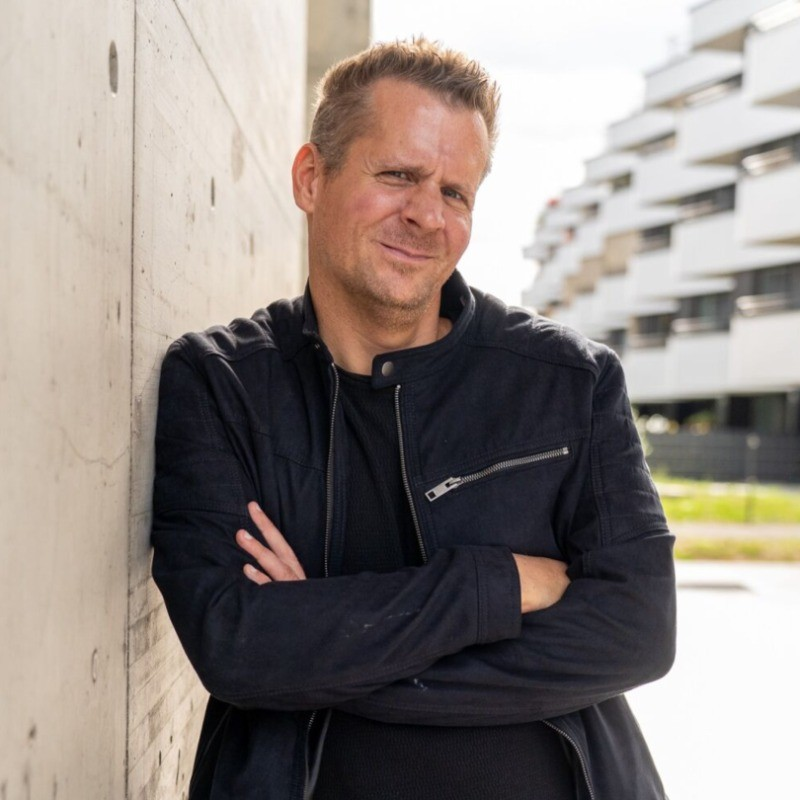
\includegraphics[width=\linewidth, keepaspectratio]{profil.jpeg}
\end{minipage}
\hfill
\begin{minipage}[t]{0.75\textwidth}
    \vspace{0pt}
    Senior Cloud Infrastructure \& DevOps Engineer mit über 9 Jahren Erfahrung in der Automatisierung von Build-Pipelines, Optimierung von Container-Workloads und dem Betrieb hochverfügbarer Softwareplattformen. M.Sc. in Scientific Computing.\\\\[0.1cm]
    Zielstrebiger Problemlöser zur Behebung kritischer Produktionsengpässe. Spezialisiert auf die Verkürzung von Release-Zyklen, Implementierung robuster Telemetrie/Monitore und die Verbindung von Dev- und Ops-Workflows durch Infrastructure as Code und automatisierte Release-Verifizierung.
\end{minipage}

\vspace{0.3cm}

\cvsection{Engineering Profile}

\colorbox{primary!10}{%
\parbox{\dimexpr\textwidth-2\fboxsep\relax}{%
    \vspace{0.10cm}
    \centering
    {\bfseries\color{primary} TECHNISCHES FUNDAMENT \& PLATFORM / DEVOPS DOMAINS\par}
    \vspace{0.08cm}

    \begin{minipage}[t]{0.31\linewidth}
        \raggedright
        \textbf{\color{primary}CI/CD \& Automation}\par
        Azure DevOps \& GitLab CI/CD\\
        Automated Testing Pipelines\\
        Release Performance Testing
    \end{minipage}
    \hfill
    \begin{minipage}[t]{0.31\linewidth}
        \raggedright
        \textbf{\color{primary}Container \& Cloud}\par
        Docker \& Containerization\\
        AWS \& Azure Cloud Services\\
        Infrastructure Automation
    \end{minipage}
    \hfill
    \begin{minipage}[t]{0.31\linewidth}
        \raggedright
        \textbf{\color{primary}Observability \& Systems}\par
        Telemetry \& Profiling Suites\\
        Linux Administration \& Bash\\
        Python \& C++ Integration
    \end{minipage}

    \vspace{0.08cm}
}%
}

\vspace{0.15cm}

{\centering
\colorbox{accent!25}{%
\parbox{\dimexpr\textwidth-25\fboxsep\relax}{%
    \vspace{0.08cm}
    \centering
    {\bfseries\color{primary}KERN-SPEZIALISIERUNG -- PLATFORM ENGINEERING\par}
    \vspace{0.05cm}
    \raggedright
    \begin{itemize}[leftmargin=1.5em, itemsep=0.15em, topsep=0.15em]
        \item \textbf{\color{primary}CI/CD Pipeline Automation:} Konzeption skalierbarer Build- und Deployment-Pipelines zur Reduzierung des Testaufwands und Beschleunigung der Markteinführung.
        \item \textbf{\color{primary}Containerization \& Cloud Operations:} Verwaltung von Docker-Container-Orchestrierung, Umgebungsstandardisierung und plattformübergreifender Infrastrukturstabilität.
        \item \textbf{\color{primary}System Profiling \& Performance Optimization:} Ursachenanalyse von Build-Engpässen, Telemetrie-Tracking und Automatisierung von Test-Suiten.
    \end{itemize}
    \vspace{0.05cm}
}%
}\par}

\cvsection{Professional Experience}

\textbf{Mindbreeze GmbH -- Quality / DevOps Engineer} \daterange{09/2022}{07/2026}\\
\textit{Python, Bash, Docker, Azure DevOps, Linux, Telemetry \& Performance Profiling \quad|\quad Team: 6 Engineers}
\begin{itemize}
    \item Entwicklung von Python/Bash-Automatisierungsframeworks, wodurch die Dauer der Release-Verifizierung von 10 auf 3 Arbeitstage reduziert wurde.
    \item Verwaltung von Docker-Container-Builds und Linux-Testinfrastruktur für Enterprise-Such-Backends.
    \item Bereitstellung automatisierter Integrations- und Regressionstests zur Überwachung der Live-Plattformleistung.
    \item Technischer Hauptansprechpartner in Release-Phasen zur Behebung von Systemengpässen und Performance-Einbußen.
\end{itemize}

\vspace{0.15cm}
\textbf{Untis GmbH -- Software Engineer (C++)} \daterange{02/2022}{06/2022}\\
\textit{C++, System Refactoring, Build Environment, Windows/Linux \quad|\quad Team: 10 Engineers}
\begin{itemize}
    \item Refactoring von Kernmodulen, Abbau technischer Schulden und Optimierung der Visual-Studio-Build-Konfigurationen.
\end{itemize}

\vspace{0.15cm}
\textbf{logi.cals -- Embedded Software Engineer (C/C++)} \daterange{02/2021}{01/2022}\\
\textit{C, C++, CI/CD Verification, Safety-Critical Architectures, Embedded Systems \quad|\quad Team: 6 Engineers}
\begin{itemize}
    \item Integration automatisierter Testverifizierungen in Build-Pipelines für sicherheitskritische Laufzeitsysteme.
\end{itemize}

\vspace{0.15cm}
\textbf{EYYES -- Software Engineer (C++/Python)} \daterange{04/2017}{12/2020}\\
\textit{Linux, Docker, CUDA, Edge Infrastructure, Real-Time Pipelines \quad|\quad Team: 8 Engineers}
\begin{itemize}
    \item Wartung von Deployment-Pipelines und Edge-Geräte-Infrastruktur für eingebettete GPU-Vision-Hardware.
    \item Automatisierung hardwarenaher Benchmarking- und Testroutinen mit Erreichung von 99,99\% Klassifikationspräzision.
\end{itemize}

\cvsection{Selected Software Projects}

\begin{itemize}[leftmargin=1.5em, itemsep=0.2em]
    \item \textbf{AWS Cloud Deep Learning Pipeline:} Cloud-native MLOps-Architektur mit automatisierten CI/CD-Inestions-Pipelines und containerisierter PyTorch-Inferenz (\href{https://github.com/CodeByMaxx/aws-pneumonia-detection}{GitHub}).\\
    \textit{Tech: AWS, Docker, Python, PyTorch, MLOps, CI/CD}
    \item \textbf{Azure AI Document Analyzer \& RAG Infra:} Skalierbare Cloud-Retrieval-Infrastruktur auf Azure mit automatisiertem Deployment und Vektordatenbankdiensten (\href{https://github.com/CodeByMaxx/AI-Document-Analyzer}{GitHub}).\\
    \textit{Tech: Azure, Docker, Vector DBs, REST APIs, Infrastructure}
    \item \textbf{Magnum C++ Game of Life:} Plattformübergreifende Build-Automatisierung und High-Performance Benchmarking-Suite für C++-Gitter-Simulationen (\href{https://github.com/CodeByMaxx/magnum-game-of-life}{GitHub}).\\
    \textit{Tech: Modern C++, CMake, Build Systems, Performance Profiling}
\end{itemize}

\cvsection{Technical Skills}

\textbf{DevOps \& Tooling:} GitLab CI/CD, Azure DevOps, GitHub Actions, Docker, Kubernetes/OpenShift, Git, Telemetry, Linux Administration.\\[0.05em]
\textbf{Scripting \& Systems:} Python, Bash, Modern C++, C, SQL, Parallel Algorithms, Multithreading.\\[0.05em]
\textbf{Cloud Platform:} Amazon AWS (S3, RDS, EC2), Microsoft Azure, Linux (Ubuntu/Debian), Microservices, REST APIs.\\[0.05em]
\textbf{Data \& Infrastructure:} PostgreSQL, DuckDB, Apache Superset, CUDA, OpenCL.

\cvsection{Education}

\textbf{M.Sc. Scientific Computing} -- Universität Wien \daterange{10/2013}{06/2017}\\
\textit{Thesis: Silent Data Corruption in FT-GMRES (\href{https://utheses.univie.ac.at/detail/40917/}{Link}, Betreuer: Prof. Dr. W. Gansterer).}

\vspace{0.1cm}
\textbf{B.Sc. Industrial Simulation} -- FH St. Pölten \daterange{09/2010}{06/2013}\\
\textit{Thesis: Simulation of Nanocomposite Materials (\href{\meinGithub/thesis/blob/master/Bakkarbeit_final.pdf}{Link}, Betreuer: Prof. Dr. T. Schrefl).}

\engineeringApproach

\cvsection{Languages \& Work Status}

\textbf{German:} Muttersprache (C2) \quad$\cdot$\quad \textbf{English:} Verhandlungssicher (C1/C2) \quad$\cdot$\quad \textbf{Work Permit:} EU-Bürger / Österreich

\end{document}
